\documentclass{standalone}
\usepackage{tikz}
\begin{document}
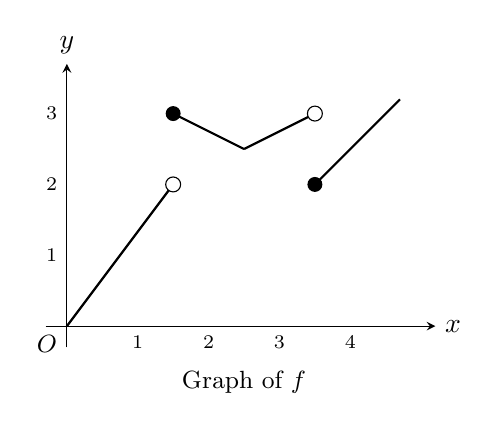
\begin{tikzpicture}[>=stealth, scale=0.9]
  % Axes
  \draw[->] (-0.3,0) -- (5.2,0) node[right] {$x$};
  \draw[->] (0,-0.3) -- (0,3.7) node[above] {$y$};

  \begin{scope}
    \clip (-0.3,-0.2) rectangle (5.1,3.6);
    % (0,1): smooth line from O to open circle at (1.5,2) — slope 4/3
    \draw[thick] (0,0) -- (1.5,2);
    % After jump: from filled dot (1.5,3), descent to corner at (2.5,2.5), slope -0.5
    \draw[thick] (1.5,3) -- (2.5,2.5);
    % After corner: ascent to open circle at (3.5,3), slope +0.5
    \draw[thick] (2.5,2.5) -- (3.5,3);
    % After second jump: from filled dot (3.5,2) going up, slope 1
    \draw[thick] (3.5,2) -- (4.7,3.2);
  \end{scope}

  % Discontinuity at x=1.5 within (1,2):
  \draw[fill=white,draw=black] (1.5,2) circle (3pt);   % open circle: left limit
  \fill[black] (1.5,3) circle (3pt);                    % filled dot: f(1.5)=3

  % Corner at (2.5,2.5) within (2,3): no special marker (continuous there)

  % Discontinuity at x=3.5 within (3,4):
  \draw[fill=white,draw=black] (3.5,3) circle (3pt);   % open circle: left limit
  \fill[black] (3.5,2) circle (3pt);                    % filled dot: f(3.5)=2

  % Axis tick labels
  \foreach \x in {1,2,3,4} {
    \node[below,font=\scriptsize] at (\x,0) {\x};
  }
  \foreach \y in {1,2,3} {
    \node[left,font=\scriptsize] at (0,\y) {\y};
  }
  \node[below left,font=\small] at (0,0) {$O$};

  % Title below
  \node[below,font=\small] at (2.5,-0.5) {Graph of $f$};
\end{tikzpicture}
\end{document}
